% !TeX spellcheck = cs_CZ
%============= Kapitola: Modulace===================================================================
\chapter{Modulace}\label{chap:ra_mod}
\minitoc

  %--------------- Rádiové komunikační systémy ----------------==-----------------------------------
  \section{Obecné schéma rádiového komunikačního systému}
    V této kapitole jsou shrnuty základní poznatky o modulacích používaných v rádiové komunikaci. 
    Nejprve se popišme obecné schéma rádiového komunikačního systému podle Shannona, které je na 
    obr. \ref{fig_RA:modulace01}. Toto schéma lze aplikovat především na systémy digitální, tedy 
    například na systémy digitálního rozhlasu a televize, na systémy digitálních celulárních 
    radiotelefonů, na systémy digitálních radiokomunikačních družicových prostředků apod. 
    \begin{figure}[ht!]  % \ref{fig_RA:modulace01}
      \centering
      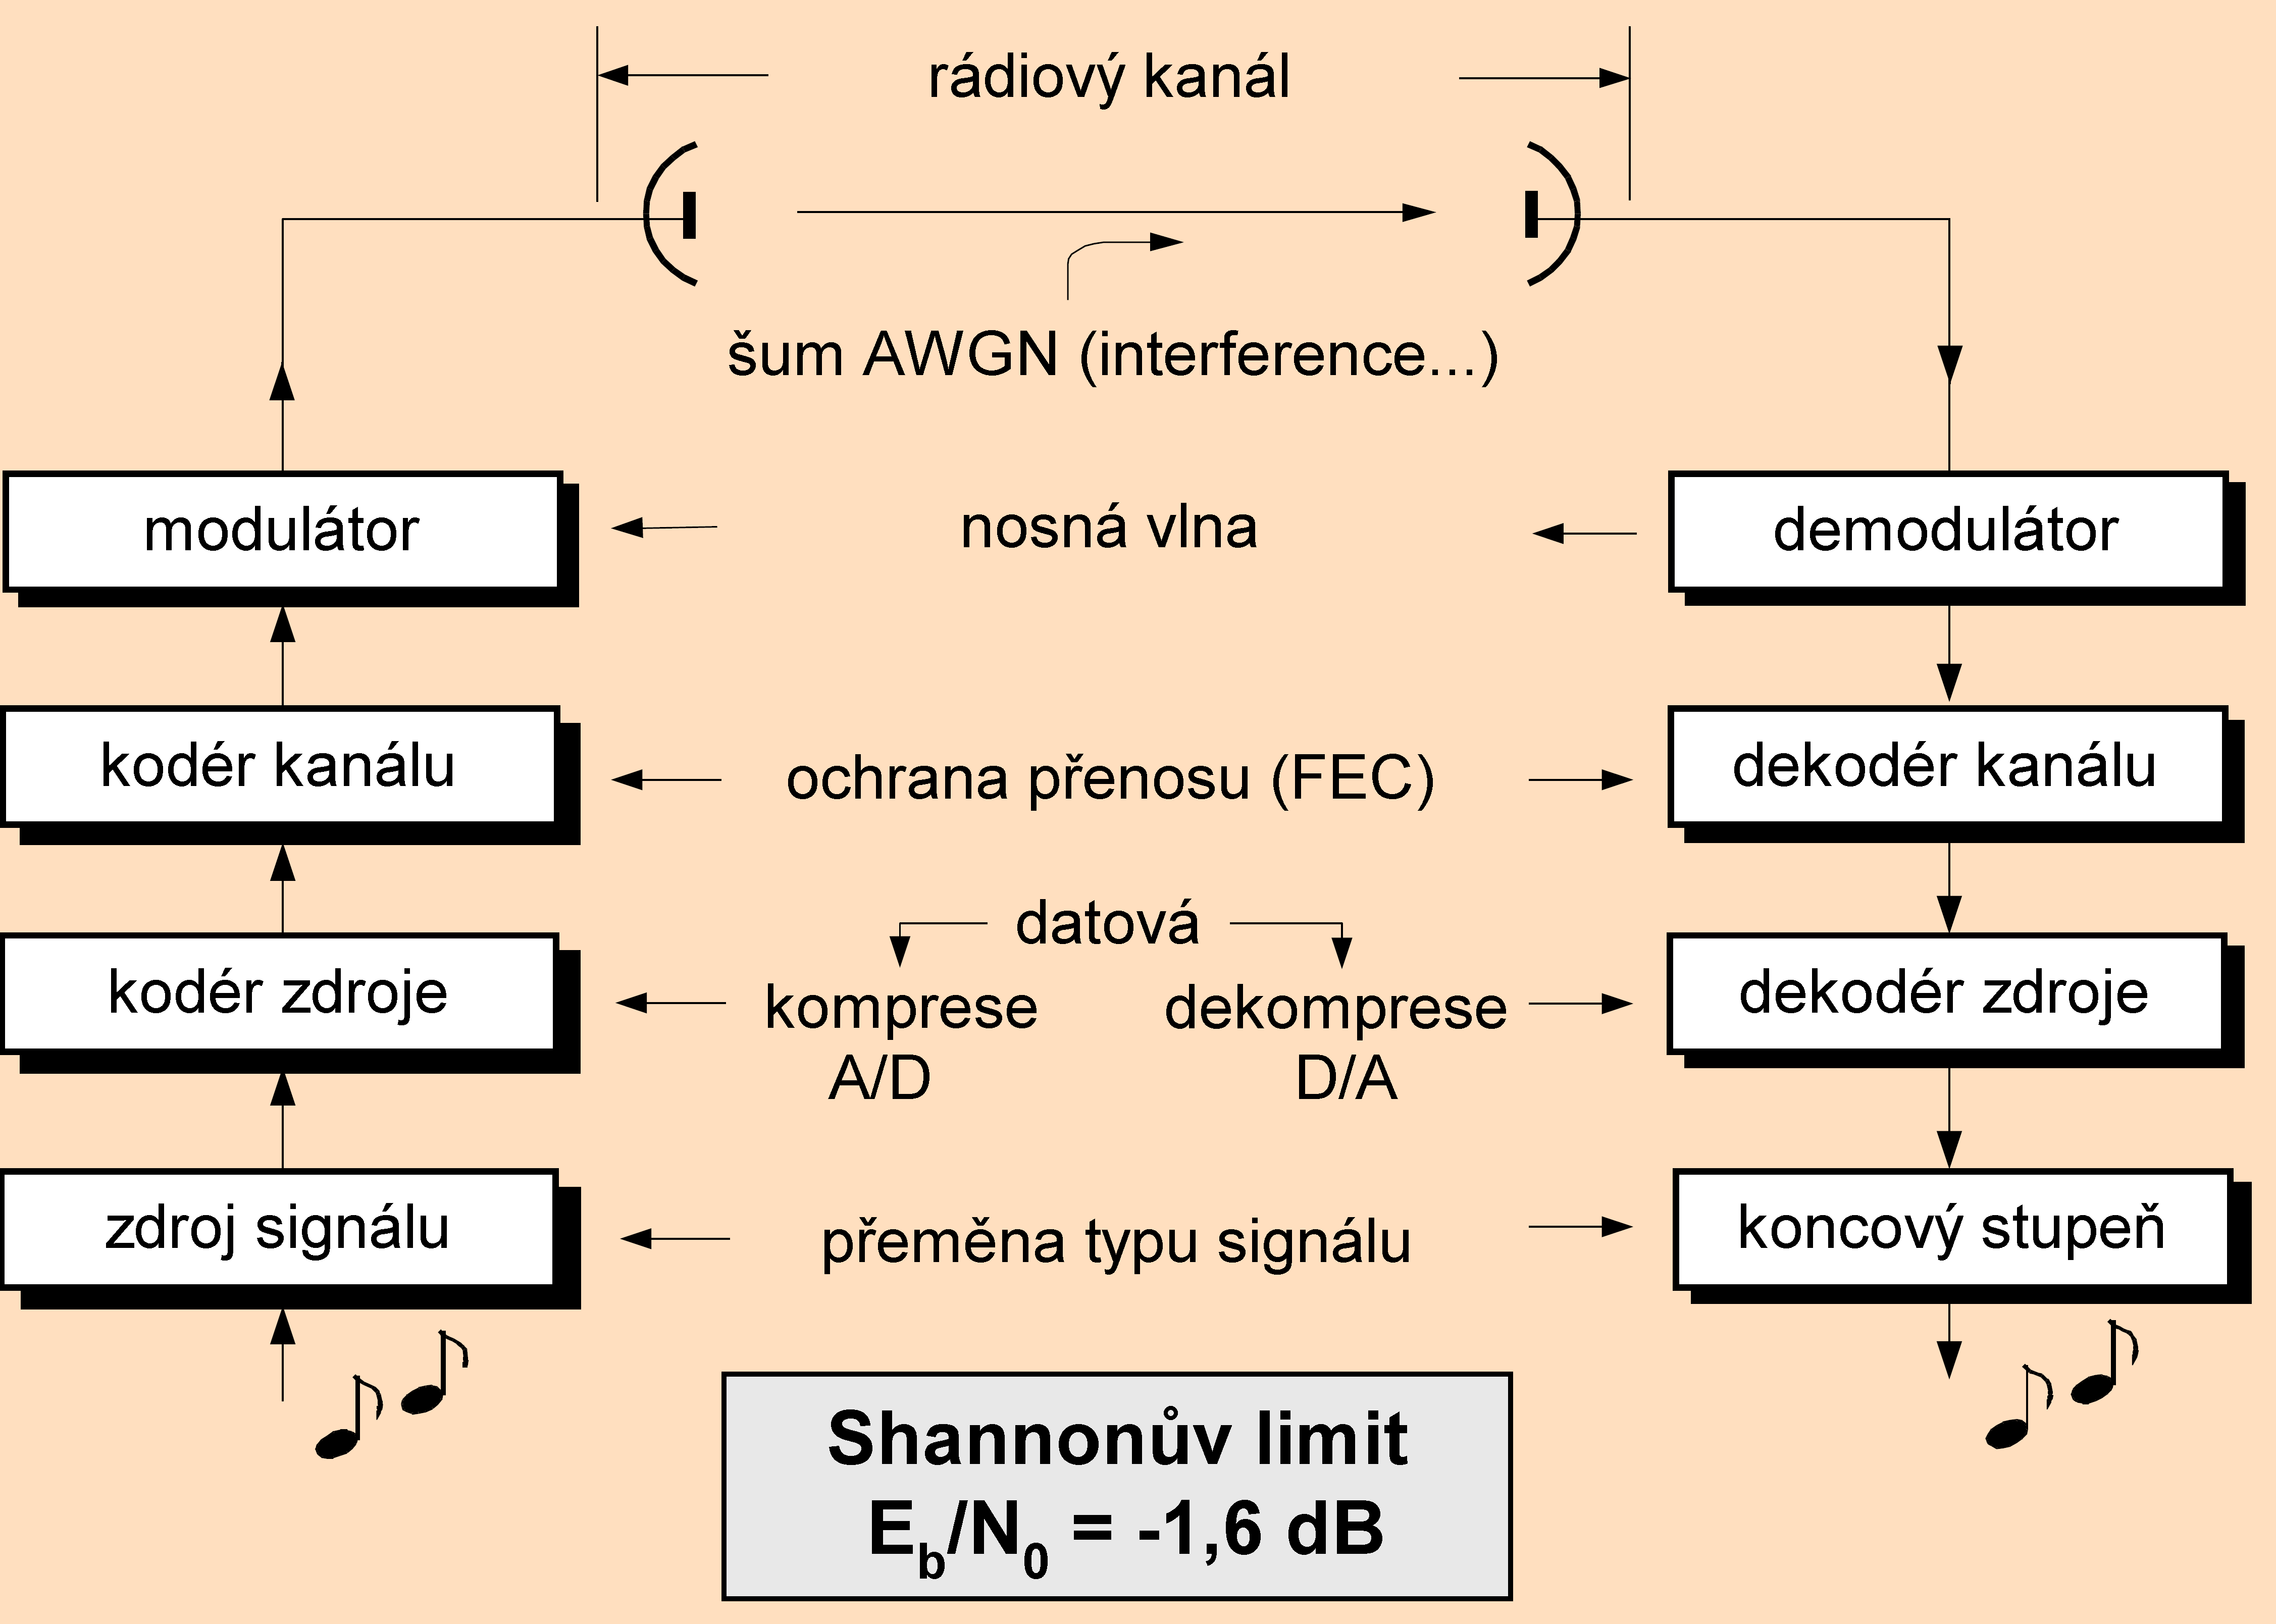
\includegraphics[width=1\linewidth]{shannon_radiokomunikacni_system.png}
      \caption{Obecné Shannonovo schéma radiokomunikačního systému
               \cite[s.~75]{ZaludRA}}
      \label{fig_RA:modulace01}
    \end{figure}
    
    Pokud se však v tomto schématu vypustí některé bloky (kodéry a dekodéry), je použitelné i pro 
    vývojově starší analogové systémy. Přestože toto schéma koncipoval Shannon již v padesátých 
    letech, je dodnes aktuální a po menších úpravách lze pomocí něho modelovat i nejmodernější 
    radiokomunikační zařízení.
    
    Na vstupu vysílače je \textbf{zdroj signálu}, jímž může být např. mikrofon nebo televizní 
    snímací elektronka apod. Ten pře\-mě\-ňu\-je přenášenou informaci, jež může mít v obecném 
    případě původně charakter neelektrické veličiny, na elektrický signál. V následujícím 
    \textbf{kodéru zdroje signálu} se signály přicházející z předchozího bloku nejprve digitalizují 
    (pokud ovšem neměly již předtím digitální podobu) a poté se podrobují vlastnímu zdrojovému 
    kódování. Tím se v nich potlačuje \emph{redundance}, což je nadbytečná informace, která je v 
    akustických, obrazových či jiných informačních tocích pocházejících z „přírodních“ zdrojů 
    většinou velmi výrazně zastoupena; (přesněji bývá redundance definována jako nadbytečnost, 
    resp. větší množství dat, než je nezbytné pro přenos informace vzhledem ke ztrátám v 
    komunikačním kanálu; dokonalá exaktní definice této veličiny je však složitá). Zde se potlačuje 
    také irelevance, volně definovaná jako nepodstatná informace. Účinnost kódování prováděného v 
    kodéru zdroje je tím lepší, čím je rychlost bitového toku na jeho výstupu nižší, než na jeho 
    vstupu; připomeňme, že proces zdrojového kódování se proto také označuje jako proces 
    \emph{komprese dat}, nebo také jako mapování vstupního digitálního signálu zdrojového kodéru na 
    jeho signál výstupní. Toto mapování se uskutečňuje podle určitého jednoznačného algoritmu. 
    Dekodér zdroje signálu na přijímací straně realizující inverzní mapování, již poskytuje na svém 
    výstupu užitečný výstupní signál, který se většinou až na zkreslení, šum a určitou složku 
    neobnovené redundance shoduje se signálem na vstupu kodéru zdroje.
        
    V následujícím \textbf{kodéru kanálu} se k binární užitečné - redundance a irelevance, alespoň 
    částečně zbavené - informační sekvenci naopak určitá \emph{redundantní} složka přidává. Je to 
    však redundance přesně kontrolovaná, která je potom využívána k potlačení rušivého působení 
    šumu a interferencí, způsobujících chybovost přenosu. V nejjednodušších (triviálních) systémech 
    kanálového kódování se prostě každý informační bit přenáší m-krát, kde \(m\) je celé kladné 
    číslo. U složitějších (netriviálních) systémů se informační tok sdružuje do sekvencí po \(k\) 
    bitech, k nimž se potom podle vhodných algoritmů přiřazují („mapují“) určité zakódované 
    sekvence po \(n\) bitech. Objem redundance, která se tímto způsobem přidává k užitečnému 
    signálu, je dán poměrem \(n/k\); reciproká hodnota tohoto poměru \(R_c = k/n\) se potom 
    označuje \emph{rychlost kanálového kódování}, nebo krátce \emph{rychlost}. \emph{Zvýšení 
    rychlosti bitového toku signálu způsobené kanálovým kódováním si bohužel vynucuje i rozšíření 
    potřebné šířky pásma komunikačního kanálu mezi vysílačem a přijímačem}.
    
    Uvedeným dvojím kódováním se získává digitální signál s potlačenou redundancí a irelevancí a se 
    zvýšenou odolností proti faktorům způsobujícím chybovost. Ten dále vchází do 
    \textbf{modulátoru}, kde se moduluje pomocí vhodného digitálního modulačního způsobu (formátu) 
    na vysokofrekvenční, nebo na mikrovlnnou nosnou vlnu. \emph{Modulace} je obecně definována jako 
    \emph{proces, při němž se některý parametr této nosné vlny (amplituda, kmitočet, fáze) mění v 
    rytmu modulačního signálu (definice podle Standardu IEEE)}. Díky využití principů modulace je 
    potom možné přenášet v určitém rádiovém prostředí, na nosných vlnách s různými kmitočty, velké 
    množ\-ství zcela nezávislých modulačních signálů. Některé typy modulací navíc umožňují v 
    procesu demodulace v přijímači zlepšit odstup užitečného signálu od šumu, i když za cenu 
    vyšších nároků na šířku pásma. Kromě toho lze při použití nosných vln o relativně vysokých 
    kmitočtech snáze realizovat vysílací i přijímací antény, účinně převádějící elektrický výstupní 
    výkon vysílačů na elektromagnetické vlny, šířící se potom rádiovým komunikačním kanálem. Zcela 
    obecně lze tedy definovat optimální modulátor jako funkční blok, který co nejlépe přizpůsobuje 
    přenášený modulační signál k parametrům následujícího rádiového komunikačního kanálu. Optimální 
    demodulátor potom naopak přijímaný signál převádí - opět pokud možno co nejvěrněji - na původní 
    modulační signál.
    
    \textbf{Komunikačním kanálem} se obecně rozumí fyzikální pros\-tře\-dí, sloužící k přenosu 
    signálu mezi vysílačem a přijímačem. V případě rádiového kanálu toto pojetí odpovídá schématu 
    na obr. \ref{fig_RA:modulace01}, někdy se však do „kanálu“ zahrnují ještě i výstupní obvody 
    vysílačů a vstupní obvody přijímačů apod., takže v zájmu jednoznačnosti je nezbytné tento 
    termín vždy přesně specifikovat. Kromě zmíněných rádiových kanálů se v praxi uplatňují také 
    vývojově vůbec nejstarší kanály s metalickými spoji používané původně v telegrafii a v 
    telefonii, v novější době potom i kanály s optickými spoji.
    
    \emph{Rádiový komunikační kanál} je specifikován určitými parametry, které mohou mít jednak 
    náhodný a jednak nenáhodný charakter. K užitečnému přenášenému signálu se zde především přidává 
    náhodný šum, o němž se v teoretických úvahách v prvém přiblížení předpokládá, že je to 
    \emph{aditivní bílý Gaussov\-ský šum \texttt{AWGN} (Additive White Gaussian Noise)} připomeňme, 
    že pojem \emph{aditivní} zde značí šum, který se lineárně sčítá s užitečným signálem, aniž by 
    docházelo ke vzájemným intermodulacím; pojem \emph{bílý} označuje šum, jehož výkonová 
    spektrální hustota je konstantní tj. nezávislá na kmitočtu a termín \emph{Gaussovský} potom 
    vyjadřuje skutečnost, že rozložení okamžitých amplitud tohoto šumu se řídí \emph{Gaussovou 
    distribucí}. Do komunikačního kanálu přicházejí dále nejrůznější náhodná \emph{rušení} tj. 
    \emph{interference}, ať již přírodního původu (atmosférické poruchy apod.), nebo pocházející od 
    „průmyslových“ zdrojů (od zapalovacích systémů automobilů, atd.). Mohou se zde však uplatňovat 
    ještě další náhodné jevy jako jsou různé typy \emph{úniků (fadingu)} apod. Kromě těchto 
    parametrů náhodného charakteru zde může být přenos signálu ovlivňován ještě dalšími efekty, 
    které mohou mít za určitých okolností nenáhodný tj. deterministický charakter. Při spojení mezi 
    stacionárním vysílačem a přijímačem takovými nenáhodnými jevy může být \emph{doba šíření 
    signálu kanálem}, jeho \emph{fázový posun} apod. Pokud jsou tyto parametry konstantní, není 
    někdy při studiu daného systému vůbec nutné znát jejich konkrétní hodnoty a dále je neuvažovat.
    
    Jedním ze základních objektivních parametrů pro hodnocení analogových komunikačních systémů je 
    jejich výstupní (po-detekční) \textbf{poměr signál/šum} tj. \(S/N\). Požadovaná hodnota tohoto 
    poměru závisí na konkrétním typu komunikačního systému a na jeho aplikaci; tak například u 
    rozhlasových přijímačů \texttt{VKV/FM} se považuje za minimum, potřebné pro jakostní příjem, 
    poměr signál/šum \SI{40}{\dB} apod. U digitálních komunikačních systémů je základním parametrem 
    obdobného významu jejich \textbf{bitová chybovost} \texttt{BER} (\emph{Bit Error Rate}), 
    definovaná jako počet chybně přenesených bitů, k celkovému počtu přenesených bitů, a to za 
    určitý dostatečně dlouhý časový interval. Nejvyšší přípustné hodnoty této ve\-li\-či\-ny 
    závisejí opět na konkrétních aplikacích. Tak například u radiotelefonních systémů postačuje při 
    přenosu hovoru chybovost \texttt{BER} řádu \num{10e-3} až \num{10e-4}, u digitální televize 
    \texttt{HDTV} musí být dosaženo podstatně nižší chybovosti řádu \num{10e-9} apod.
    
    V původním Shannonově schématu jsou na vysílací straně uvažovány kodér kanálu a modulátor po 
    funkční i realizační stránce jako dva zcela samostatné bloky. Později se však ukázalo, že v 
    některých systémech je vhodné proces ka\-ná\-lo\-vé\-ho kódování a modulace funkčně sdružit. 
    Tím se vytvoří tzv. \textbf{kódované modulace}, které se začínají v moderní rádiové komunikaci 
    v devadesátých letech stále výrazněji prosazovat. Ty mají velkou přednost hlavně v tom, že 
    nevyžadují znatelné zvětšení šířky pásma komunikačního kanálu, které si naopak v klasickém 
    Shannonově systému vynucuje izolované kanálové kódování. \cite[s.~75]{ZaludRA}
    
    \subsection{Přenosová kapacita rádiového komunikačního systému}
      Libovolný rádiový komunikační systém podle obr. \ref{fig_RA:modulace01} nemůže přenést v 
      určitém časovém intervalu zcela libovolné, neomezené množství informace, nýbrž pouze množství 
      nepřesahující jeho \textbf{přenosovou kapacitu} \(C\). V každém reálném systému je totiž 
      přítomen šum a řada dalších rušivých jevů, které ztěžují na přijímací straně vyhodnocování 
      relativně velmi malých užitečných signálů. Předpokládejme dále, že v radiokomunikačním kanálu 
      tohoto systému působí \emph{pouze} aditivní bílý Gaussovský šum \texttt{AWGN}. Přenosová 
      kapacita \(C\) je potom \emph{definována jako maximální množství informace vyjádřené v 
      bitech, jež může být daným systémem přeneseno za určitý časový interval, např. za \(1\) 
      sekundu, a to při nulové (přesněji řečeno libovolně malé) chybovosti \texttt{BER}}; pokud se 
      v systému 
      uplatňuje snaha tento horní limit překročit, chybovost prudce narůstá. Označí-li se 
      \emph{střední hodnoty výkonu užitečného signálu} na vstupu přijímače symbolem \(S\) a 
      \emph{šumu} symbolem \(N\) a \emph{šířka pásma} daného kanálu \(B\), je kapacita \(C\) určena 
      \textbf{Shannonovým - Hartleyovým vztahem}
      \begin{subequations}
        \label{eq:RA_shannon_C01}
        \begin{align}
          C &= B\log_2\left(1+\frac{S}{N}\right),\,\text{resp.}    \label{eq:RA_shannon_C01a} \\ 
          C &= 3,32\cdot B\log_{10}\left(1+\frac{S}{N}\right)      \label{eq:RA_shannon_C01b}
        \end{align}
      \end{subequations}
      Připomeňme, že poměr signál/šum na vstupu přijímače se nejčastěji označuje symbolem \(C/N\) 
      \emph{(Carrier/Noise)}, kdežto symbol \(S/N\) značí poměr signál/šum až za demodulátorem 
      \emph{(Signal/Noise)}
      
      Kapacita \(C\) vyjadřuje maximální dosažitelnou rychlost přenosu informace idealizovaným 
      radiokomunikačním systémem, v němž působí jen výše zmíněný aditivní bílý Gaussovský šum 
      \texttt{AWGN}, a to při chybovosti \texttt{BER} blížící se k nule. Dále se předpokládá, že je 
      zde použito \emph{optimální kódování} a \emph{optimální modulace}. Reálné systémy se mohou 
      této kapacitě pouze přiblížit, a to tím dokonaleji, čím věrněji se v nich použité metody 
      kódování a modulace přibližují metodám optimálním. Přitom je nutné zdůraznit, že tyto zcela 
      dokonalé optimální metody nejsou v praxi dosažitelné, přičemž pokusy o jejich realizaci vedou 
      k rapidnímu nárůstu složitosti příslušných technických prostředků.
      
      Požadovanou kapacitu \(C\) je možné v praxi dosáhnout různými kombinacemi parametrů \(B, S\) 
      a \(N\). U pozemských radiokomunikačních systémů ji lze často získat použitím velkých výkonů 
      vysílačů, antén s velkým ziskem apod., tedy velkým poměrem \(S/N\), takže se zde potom 
      vystačí s relativně malými šířkami pásma B. Naproti tomu například pro družicové systémy jsou 
      typické malé výkony palubních vysílačů, takže požadovanou kapacitu \(C\) je možné získat 
      jedině náležitým rozšířením pásma \(B\).
      
      Kapacita \(C\) určená vztahem (\ref{eq:RA_shannon_C01}) je závislá na třech veličinách \((B, 
      S, N)\). Vyjádří-li se v tomto vztahu výkon šumu \(N\) jako \emph{součin spektrální výkonové 
      šumové hustoty} \(N_0\) a \emph{šířky pásma} \(B\), tedy \(N = N_0\cdot B\) a zavede-li se do 
      něho poměrná šířka pásma \(B_0 = S/N_0\), lze ho přepsat do normovaného tvaru 
      \begin{equation}\label{eq:RA_shannon_C02}
        \frac{C}{B_0} = \frac{B}{B_0}\log_2\left(1+\frac{B_0}{B}\right)
      \end{equation}
      
      Zde je \textbf{normovaná přenosová kapacita} \(C/B_0\) vyjádřena již jen jako funkce jediné 
      proměnné, a to \emph{poměrné šířky pásma} \(B/B_0\). Tato funkce je zobrazena v grafu na obr. 
      \ref{fig_RA:modulace02}. V tomto grafu je rovněž zobrazena závislost poměru \emph{signál/šum} 
      = \(S/N\) na poměrné šířce pásma \(B/B_0\), pro kterou z rovnosti posledních členů relací 
      (\ref{eq:RA_shannon_C01}) a (\ref{eq:RA_shannon_C02}) vyplývá vztah      
      \begin{equation}\label{eq:RA_shannon_C03}
        \frac{S}{N} = \frac{1}{B/B_0}
      \end{equation}      
      
      \begin{figure}[ht!]  % \ref{fig_RA:modulace02}
        \centering
        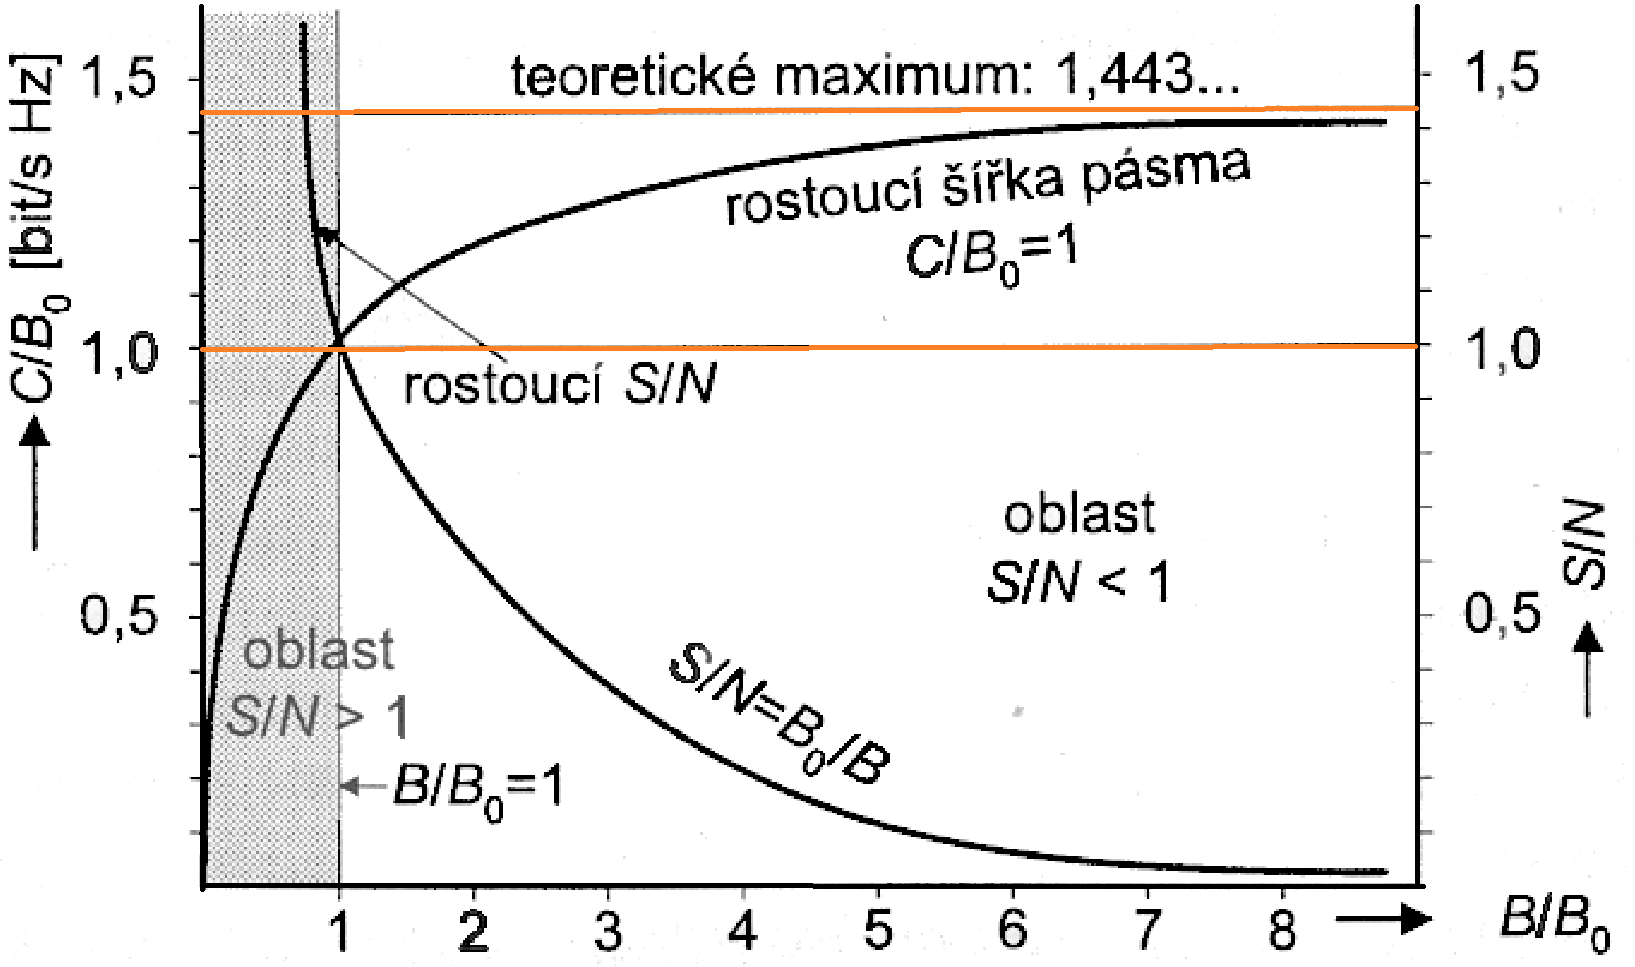
\includegraphics[width=0.8\linewidth]{shannon_graf_C_N.png}
        \caption{Závislost normované přenosové kapacity \(C/B_0\) na poměru signál/šum - \(S/N\)  
                 rádiového komunikačního systému na normované šířce pásma \(B/B_0\)
                  \cite[s.~79]{ZaludRA}}
        \label{fig_RA:modulace02}
      \end{figure} 
      
      Normovaná šířka pásma \(B/B_0\) odpovídá stavu, kdy se výkon signálu \(S\) rovná výkonu šumu 
      \(N\). Svislice vedená bodem \(B/B_0 = 1\) na vodorovné ose potom dělí celý graf na dvě 
      části. Levá, zvýrazněná část odpovídá klasickým radiokomunikačním systémům, které pracují při 
      poměru signál/šum podstatně větším než jedna, přičemž jejich normovaná přenosová kapacita je 
      hluboko pod dosažitelným maximem \(C/B_0 = 1,443\). Pravá část pak odpovídá perspektivním 
      „širokopásmovým“ radiokomunikačním systémům, které naopak pracují při poměru signál/šum \( 
      S/N\ll1\), avšak s přenosovou kapacitou blížící se dosažitelnému maximu \(\num{1.443}\). Tyto 
      systémy se označují také jako \textbf{systémy s rozprostřeným spektrem}, nebo \emph{systémy s 
      kódovým multiplexem \texttt{CDMA} (Code Division Multiple Access)}. Jejich realizace je 
      obecně podstatně složitější, než realizace systémů klasických a bez vyspělé monolitické 
      technologie by byla v praxi velmi obtížná. Na druhou stranu však mají systémy druhé kategorie 
      výhodu velice efektivního využití kmitočtového spektra, které totiž mohou sdílet s jinými 
      radiokomunikačními službami aniž by se vzájemně rušily. Mezi jejich další hlavní přednosti 
      náleží možnost dobře pracovat v radiokomunikačních kanálech s vysokou úrovní poruch nebo i 
      úmyslného rušení, dále schopnost účinně potlačovat úniky signálu a konečně i schopnost 
      poměrně spolehlivě utajit přenos před nepovolanými subjekty.\cite[s.~78]{ZaludRA}
     
      
  \section{Modulace a jejich klasifikace}
    V rádiové komunikaci se používá větší počet různých typů (formátů) modulací. Jejich základní 
    klasifikace, vycházející z časového vývoje, je uvedena na obr \ref{fig_RA:modulace03}. Vývojově 
    nejstarší jsou \emph{analogové modulace}. Později se začaly uplatňovat i \emph{diskrétní 
    modulace}, a to nejprve v základním pásmu a potom i v oblasti vysokofrekvenční. Diskrétní 
    modulace v základním pásmu byly nejprve \emph{nekódované}, za nimi potom následovaly i modulace 
    \emph{kódované}. Nejmladší jsou potom \emph{diskrétní modulace s nosnými vlnami}, které pro 
    stručnost dále nazýváme \emph{modulace digitální}. Uveďme si podrobnější klasifikaci všech 
    zmíněných variant. \cite[s.~82]{ZaludRA}
    \begin{figure}[ht!]  % \ref{fig_RA:modulace03}
      \centering
      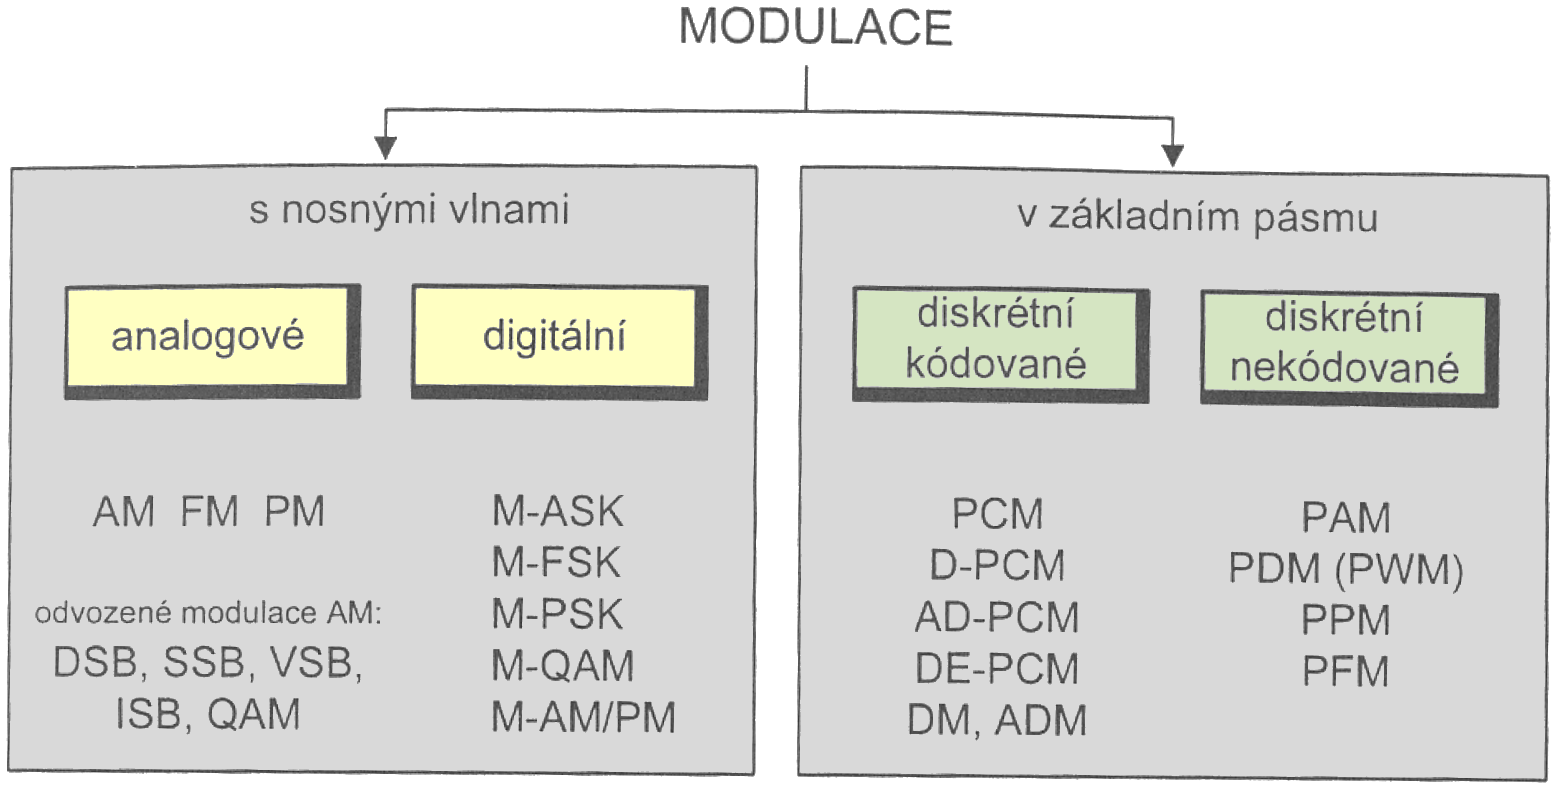
\includegraphics[width=0.9\linewidth]{modulace_prehled.png}
      \caption{Přehled modulačních způsobů používaných v rádiové komunikaci
                \cite[s.~82]{ZaludRA}}
      \label{fig_RA:modulace03}
    \end{figure}
    
    \subsection{Klasifikace analogových modulací}
      Analogové modulace vznikají tak, že se pomocí analogového modulačního signálu (tedy signálu 
      spojitého v čase i v amplitudě) moduluje analogová sinusová vysokofrekvenční nebo mikrovlnná 
      nosná vlna. Modulací se přitom rozumí ovlivňování některého parametru (charakteristické 
      veličiny) nosné vlny modulačním signálem. Je-li to amplituda, vznikne \emph{amplitudová 
      modulace \texttt{AM} (Amplitude Modulation)}, při ovlivňování kmitočtu se vytváří 
      \emph{kmitočtová modulace \texttt{FM} (Frequency Modulation)} a při ovlivňování fáze se 
      vytváří \emph{fázová modulace \texttt{PM} (Phase Modulation)}.
      
      Amplitudově modulovaný signál má kmitočtové spektrum, obsahující nemodulovanou nosnou vlnu a 
      dvě postranní kmitočtová pásma, nesoucí informaci. Určitými modifikacemi tohoto spektra potom 
      vznikají různé vývojově mladší varianty amplitudové modulace \texttt{AM}. 
      \begin{itemize}
        \item \emph{\texttt{AM} s oběma postranními pásmy \texttt{DSB} (Double Side Band)}: jsou 
               přenášena obě postranní pásma, avšak nosná je částečně nebo zcela potlačena,
        \item \emph{\texttt{AM} s jedním potlačeným postranním pásmem \texttt{SSB} (Single Side 
               Band)}: přenos jediného postranního pásma a úplně, nebo alespoň částečně potlačené 
               nosné vlna
        \item \emph{\texttt{AM} s jedním částečně potlačeným postranním pásmem \texttt{VSB} 
               (Vestigial Side Band)}: přenosu jednoho kompletního a jednoho částečně potlačeného 
               postranního pásma. Má obvykle nepotlačenou nosnou vlnu 
        \item \emph{\texttt{AM} s nezávislými postranními pásmy \texttt{ISB} (Independent Side 
               Band)}:Nosná vlna zcela nebo částečně potlačena a v každém úplném postranním pásmu 
               se přenáší nezávislý modulační signál.
        \item \emph{Analogová kvadraturní amplitudová modulace \texttt{QAM} (Quadrature Amplitudě 
               Modulation)}: používá dvě nosné vlny, které mají přesně shodné kmitočty, avšak 
               jejich fázový posuv je trvale \SI{90}{\degreeCelsius}. Každá z těchto nosných vln je 
               amplitudově modulována nezávislým modulačním signálem, přičemž může být částečně 
               nebo zcela potlačena.
      \end{itemize}
      
      Má-li být u předchozích modulací zdůrazněno, že je u nich zcela potlačena nosná vlna, bývá 
      jejich označení ještě doplněno zkratkou \emph{\texttt{SC} (Supressed Carrier)}, tedy 
      například \texttt{DSB-SC}, \texttt{SC-DSB}, nebo \texttt{DSB\textsubscript{SC}}.
      
    \subsection{Diskrétní nekódované modulace v základním pásmu}
      Základním typem této kategorie je \emph{pulzní amplitudová modulace \texttt{PAM} (Pulse 
      Amplitude Modulation)}. Ta vzniká ve své nejjednodušší podobě tak, že se analogový modulační 
      signál přivádí na klíčovaný spínač, který je spínán sledem pravoúhlých impulzů. Za spínačem 
      se potom již objevuje signál \texttt{PAM}, a to v podobě sekvence v čase nespojitých impulzů, 
      jejichž amplitudy kopírují průběh analogového modulačního signálu \cite[s.~84]{ZaludRA}.
      
      Kromě změn amplitudy se u impulzové nosné vlny dají měnit i jiné parametry viz obr. 
      \ref{fig_RA:modulace04}:
      \begin{itemize}
        \item \emph{diskrétní šířková modulace \texttt{PDM}, resp. \texttt{PWM} (Pulse Duration  
              Modulation resp. Pulse Width Modulation)}: změnou šířky impulzů impulzové nosné vlny,
        \item \emph{diskrétní polohová modulace \texttt{PPM} (Pulse Position Modulation)}: změnou  
              polohy impulzů uvažované impulzové nosné vlny, vůči poloze nominální
        \item \emph{diskrétní kmitočtová modulace \texttt{PFM} (Pulse Frequency Modulation)}:  
              změnou kmitočtu této nosné.
      \end{itemize} 
    \subsection{Diskrétní kódované modulace v základním pásmu}
      Nejrozšířenějším typem z této kategorie je \emph{impulzová kódovaná modulace \texttt{PCM} 
      (Pulse Code Modulation)}. Ta se vytváří tak, že se analogový modulační signál nejprve přemění 
      na signál \texttt{PAM}. Ten se poté podrobuje \emph{kvantování}; přitom se jeho celý 
      dynamický rozsah rozdělí na konečný počet \emph{kvantizačních úrovní (hladin)} a každé 
      skutečné úrovni impulzu \texttt{PAM} se přiřadí určitá (například nejbližší) úroveň 
      kvantizační (diskrétní). Kvantovaný signál \texttt{PAM} se dále kóduje. Kódováním se rozumí 
      převod (mapování) jeho skutečné velikosti - vyjádřené obvykle v desítkové soustavě - do 
      soustavy binární (nebo jiné, mající nižší číselný základ, než původní soustava desítková). 
      Tím se vytvoří signál s modulací \texttt{PCM}.
      \begin{itemize}
        \item \emph{diferenční \texttt{D-PCM} (Differentially - \texttt{PCM})}: nekóduje se 
              skutečná velikost kvantovaných vzorků PAM, nýbrž pouze rozdíl mezi touto skutečnou 
              velikostí a velikostí predikovanou (tj. předpověděnou z několika předchozích 
              kvantovaných vzorků).
        \item \emph{diferenciálně kódované \texttt{DE-PCM} (Differentially encoded —
              \texttt{PCM})}: nejprve se vytváří signál \texttt{PCM}; z něho se potom pomocí 
              vhodného algoritmu získává signál \texttt{DE-PCM}, u něhož je informace obsažena 
              nikoliv v samotné logické hodnotě příslušného bitu signálu \texttt{PCM}, nýbrž v 
              rozdílu tohoto bitu oproti hodnotě bitu předchozího.
        \item \emph{delta modulace \texttt{DM} (Delta Modulation)}: v podstatě představuje   
              jednobitovou variantu modulace \texttt{PCM}; je-li \(w\)-tý vzorek analogového 
              modulačního signálu větší než vzorek předchozí, je v signálu \texttt{DM} bit \(1\) a 
              je-li tento vzorek menší než předchozí, je v signálu \texttt{DM} bit \(0\).
      \end{itemize}
      
      Všechny předchozí varianty diskrétních kódovaných modulací pracují s konstantním kvantizačním 
      krokem. U \emph{adaptivní modulace \texttt{D-PCM} tj. \texttt{AD-PCM}} a rovněž u 
      \emph{adaptivní modulace \texttt{DM} tj. \texttt{A-DM}}, se kvantizační krok naopak mění v 
      závislosti na průběhu analogového modulačního signálu.
    
    \begin{figure}[ht!]  % \ref{fig_RA:modulace04}
      \centering
      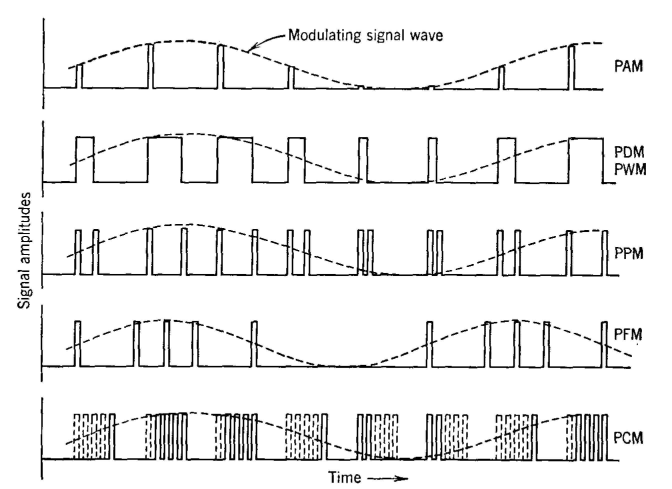
\includegraphics[width=1\linewidth]{modulace_zakladni_pasmo.png}
      \caption{Přibližné tvary a uspořádání signálů diskrétních pulsní modulací pro sinusový   
               modulační signál (tečkovaná křivka). Výška impulsů obecně neodpovídá výšce modulační 
               vlny.}
      \label{fig_RA:modulace04}
    \end{figure}
    
    \subsection{Digitální modulace (diskrétní modulace s nosnými vlnami)}
      Tyto modulace vznikají tak, že se vysokofrekvenční nebo mikrovlnná sinusová nosná vlna 
      moduluje signálem některé diskrétní modulace v základním pásmu; jedná se zde tedy vlastně o 
      dvojnásobnou modulaci, neboť modulačním signálem je již předtím modulovaný signál. K modulaci 
      se používá většinou binární signál \texttt{PCM}, nebo jeho některé modifikace, ostatní 
      diskrétní modulace se k danému účelu používají jen zřídka.
      
      Binárním modulačním signálem je možné modulovat amplitudu, kmitočet anebo fázi nosné vlny. U 
      \emph{dvoustavových modulací} se modulovaný parametr této vlny mění pouze mezi dvěma 
      diskrétními stavy, z nichž jeden odpovídá modulačnímu bitu 0 a druhý bitu 1. Tyto diskrétní 
      stavy nosné vlny se u digitálních modulací označují obecně termínem \emph{signálové prvky} 
      resp. \emph{symboly}, okamžiky přechodu mezi nimi se potom nazývají \emph{charakteristické 
      okamžiky}. Pro uvažované digitální modulace se používá rovněž termín \textbf{klíčování}; 
      (změny nosné vlny mezi několika diskrétními stavy se tímto slovem označují vlastně již od 
      počátků radiokomunikace, nejprve zřejmě ve spojení „klíčovaná telegrafie“).
      \begin{itemize}
        \item \emph{dvoustavové klíčování amplitudovým zdvihem \texttt{2-ASK} (Amplitudě Shift  
              Keying)}: klíčováním amplitudy nosné vlny, se získá dvoustavová modulace 
              \texttt{PCM-AM}
        \item \emph{dvoustavové klíčování kmitočtovým zdvihem \texttt{2-FSK} (Frequency Shift  
              Keying)}: klíčování kmitočtu nosné vlny se vytváří dvoustavová modulace 
              \texttt{PCM-FM},
        \item \emph{dvoustavové klíčování fázovým zdvihem \texttt{2-PSK}, (Phase Shift Keying)}: 
              klíčování fáze nosné vlny potom konečně vzniká dvoustavová modulace \texttt{PCM-PM}.
      \end{itemize}
      U dvoustavových modulací odpovídá každý modulační stav modulované nosné vlny jedinému bitu 
      modulačního signálu \texttt{PCM}. Snaha po zvětšení přenosové kapacity digitálních modulací 
      však vedla k rychlému rozvoji \emph{vícestavových diskrétních modulací}, u nichž každý 
      signálový prvek modulované nosné vlny přenáší nejméně dva, nebo i více bitů. Tak například u 
      \emph{čtyřstavové modulace \texttt{4-FSK (Q-FSK)}} tato vlna zaujímá čtyři diskrétní 
      kmitočty; každá z nich zde však již nereprezentuje jediný bit jako v případě modulace 
      \texttt{2-FSK}, nýbrž dva bity, tj. \emph{bitovou dvojici}, nazývanou také \emph{dibit}. 
      Analogicky   \emph{čtyřstavová modulace \texttt{4-PSK (Q-PSK)}} pracuje se čtyřmi diskrétními 
      fázovými 
      stavy nosné vlny, z nichž každý odpovídá určitému dibitu modulačního signálu atd. Rychlost, 
      se kterou se mění diskrétní stavy nosné vlny se nazývá \textbf{symbolová rychlost} \(f_s\) 
      tato rychlost se vyjadřuje v jednotkách \emph{baud \textbf{[Bd]}}, přičemž je rovna reciproké 
      hodnotě doby trvání \(T_s\) signálového prvku, tedy\[f_s = \frac{1}{T_s}.\]
      
      U čtyřstavových modulací \texttt{4-ASK}, \texttt{4-FSK} a \texttt{4-PSK} zřejmě každý 
      signálový prvek přenáší dva bity, proto je zde symbolová rychlost \(f_s\) rovna právě jedné 
      polovině bitové rychlosti \(f_b\) V důsledku toho je potom i potřebná šířka pásma 
      vy\-so\-ko\-frek\-ven\-ční\-ho kanálu u těchto modulací poloviční, v porovnání s modulacemi 
      dvoustavovými (ovšem při téže bitové rychlosti modulačního signálu \texttt{PCM}). U 
      osmistavových modulací nese každý signálový prvek informaci již o třech bitech (tj. o jednom 
      \textbf{tribitu}), což vede pouze ke třetinové šířce pásma vysokofrekvenčního kanálu. Obecně 
      potom platí, že u modulace s \(M\) stavy přenáší každý symbol informaci o \(n = \log_2 M\) 
      bitech. Šířka pásma \(B_M\) kanálu obecné \emph{M-stavové modulace}, v závislosti na šířce 
      pásma \(B_2\) základní dvoustavové modulace, je tedy určena vztahem \(B_M = \frac{B_2}{\log_2 
      M}.\) 
      
      Vývojově mladší kategorii digitálních modulací potom představují \emph{M-stavové modulace se 
      současným klíčováním amplitudy a fáze nosné vlny}, značené původně symbolem 
      \texttt{M-ASK/PSK}; pro tyto modulace je však již běžnější označení \emph{M-stavové 
      kvadraturní amplitudové modulace \texttt{M-QAM}\footnote{nezaměňovat s analogovou kvadraturní 
      modulací \texttt{QAM}, popisovanou výše} (Quadrature Amplitude Modulation)}.
      
      Od počátku devadesátých let se dostávají do praxe také již zmíněné \emph{kódované modulace}, 
      které vznikají spojením kanálového kódování a vlastní modulace do jediného procesu, 
      realizovaného v jediném funkčním bloku. 
    
    \subsection{Lineární modulace a nelineární modulace, modulace s pamětí a bez paměti}
      Předchozí klasifikace modulací vychází z jejich historického vývoje, přičemž rozlišuje 
      jednotlivé modulace na základě různých typů modulačních signálů a rozdílných modulovaných 
      parametrů nosné vlny.
      
      Dělení na \textbf{lineární} a \textbf{nelineární modulace} se uplatňuje především u modulací 
      s nosnými vlnami. \emph{Analogové lineární modulace} jsou takové, u nichž je amplituda nosné 
      vlny danou, obecně lineární funkcí okamžitých hodnot modulačního signálu. U lineárních 
      modulací Platí \emph{princip superpozice} mezi různými složkami kmitočtového spektra 
      modulovaného signálu, příslušejícími různým složkám spektra modulačního signálu. Do této 
      kategorie patří amplitudová modulace AM i všechny její varianty, tj. modulace \texttt{DSB}, 
      \texttt{SSD} atd. U \emph{analogových nelineárních modulací} zmíněná lineární závislost 
      amplitudy nosné na modulačním signálu neexistuje a princip superpozice neplatí, takže ve 
      spektru modulovaného 
      signálu jsou přítomny také \emph{intermodulační produkty} základních složek. Sem náležejí dvě 
      kategorie tzv. \emph{exponenciálních modulací}, a to \emph{kmitočtová modulace \texttt{FM}} a 
      \emph{fázová modulace \texttt{PM}}; tyto modulace jsou charakterizovány \emph{konstantní 
      obálkou nosné vlny}. U \emph{diskrétních lineárních modulací} při mapování modulačního 
      digitálního signálu (informační datové sekvence), do po sobě následujících stavů (signálových 
      prvků) modulované nosné vlny, platí princip superpozice. U \emph{diskrétních nelineárních 
      modulací} naopak princip superpozice mezi po sobě následujícími stavy modulovaného signálu 
      neplatí. Tyto   modulace mohou, ale také nemusí mít konstantní obálkou modulované nosné vlny, 
      v závislosti na tom zda se u nich netvaruje - nebo tvaruje modulační datová sekvence.
      
      U \textbf{digitálních modulací s pamětí} určitý stav nosné vlny závisí nejen na jemu 
      odpovídajícím bloku (kódové skupině) binárního modulačního signálu, nýbrž určitým způsobem i 
      na předchozích stavech této vlny, resp. na předchozích blocích modulačního signálu. Uvedená 
      závislost zde vzniká zpravidla již na úrovni modulačních signálů, které se totiž z původní 
      vstupní podoby nejprve překódují do podoby „s pamětí“ a teprve poté se přivádějí na 
      modulátor. U \textbf{digitálních modulací bez paměti} se tato závislost neobjevuje.
      
      Výše uvedené kategorie se mohou vzájemně kombinovat, čímž vznikají celkem čtyři možné 
      varianty, které se striktně rozlišují především u digitálních modulací. K lineárním modulacím 
      bez paměti náležejí například formáty \texttt{2-PSK, 4-PSK,} k lineárním modulacím s pamětí 
      formáty \texttt{DE-PSK, \(\pi\)/4-QPSK} atd. 
      
      Poslední klasifikace se týká pouze modulací, u nichž je modulační signál \emph{nespojitý 
      (diskrétní) v čase}. \textbf{Koherentní modulace} jsou takové, u nichž existuje předem určený 
      vztah mezi okamžiky charakterizujícími fázi nosné vlny před modulací a charakteristickými 
      okamžiky modulovaného signálu. Do této kategorie náležejí například modulace, u nichž 
      charakteristické okamžiky modulovaného signálu splývají s průchody nosné vlny nulou 
      (konkrétně je to např. modulace MSK apod.). Modulace, u nichž předem určený vztah mezi fází 
      nosné vlny a charakteristickými okamžiky modulovaného signálu neexistuje, se nazývají 
      \textbf{modulace nekoherentní}.
      
  \section{Analogové modulace}
    Vývojově nejstarší systémy pro pozemskou radiokomunikaci používaly pro přenos analogovou 
    amplitudovou modulaci \texttt{AM}, k níž se později připojila analogová kmitočtová modulace 
    \texttt{FM} a fázová modulace \texttt{PM}. Modulace \texttt{AM} a její varianty se v současné 
    době uplatňují spíše už jen u jednodušších systémů, jako je například rozhlas \texttt{AM}, 
    občanské radiostanice apod. Naproti tomu modulace \texttt{FM} stále ještě nachází využití i v 
    náročnějších aplikacích jako je stereofonní rozhlas \texttt{FM} apod \cite[s.~75]{ZaludRA}.
    
    \subsection{Základní principy analogových modulací}
      U analogových modulací se obecným modulačním signálem \(m(t)\) moduluje vhodný parametr 
      spojité, harmonické (např. kosinusové) vysokofrekvenční nosné vlny. Modulační signál může mít 
      charakter napětí nebo proudu, v dalším však většinou předpokládáme, že je to signál napěťový. 
      Modulované napětí lze potom vyjádřit obecným vztahem
      \begin{equation}\label{eq:RA_mdlc_01}
        u_{mod}(t) = u_i(t)\cos[\Phi_i(t)]
      \end{equation}
      kde \(u_i (t)\) je \emph{okamžitá amplituda} napětí modulované nosné vlny; \(\Phi_i(t)\) 
      okamžitá fáze modulované nosné vlny.
      
      Mění-li se amplituda napětí \(u_i(t)\) modulované nosné vlny lineárně s modulačním napětím 
      \(m(t)\), přičemž okamžitá fáze \(\Phi_i(t)\) zůstává konstantní, získá se \emph{amplitudová 
      modulace}, která náleží do kategorie \emph{lineárních modulací}. U lineárních modulací jsou v 
      kmitočtovém spektru modulovaného signálu obsaženy jen složky, které odpovídají jednotlivým 
      harmonickým složkám modulačního signálu.
      
      Jestliže se u modulované nosné vlny mění podle určitého zákona okamžitá fáze \(\Phi_i(t)\) s 
      modulačním napětím \(m(t)\), přičemž amplituda zůstává konstantní, vytvářejí se \emph{úhlové 
      (exponenciální) modulace}, náležející do kategorie \emph{nelineárních modulací}. V jejich 
      kmitočtovém spektru jsou nejen složky odpovídající jednotlivým harmonickým modulačního 
      signálu, nýbrž i jejich vzájemné intermodulační produkty. Z nich je nejčastěji využívána 
      \emph{kmitočtová modulace \texttt{FM}}, u níž je okamžitá odchylka kmitočtu (tj. derivace 
      fáze podle času) modulované nosné vlny, vůči kmitočtu nemodulované nosné vlny, úměrná 
      modulačnímu signálu. K exponenciálním modulacím náleží dále \emph{fázová modulace 
      \texttt{PM}}, u níž je okamžitá odchylka fáze, od fáze nemodulované nosné vlny, úměrná 
      modulačnímu signálu. Modulace \texttt{FM} a \texttt{PM} mají konstantní obálku modulované 
      nosné vlny. To je v praxi výhodné, neboť signály s konstantní obálkou mohou být zesilovány 
      výkonovými zesilovači nastavenými do nelineární pracovní třídy C (D, E, ...), vyznačující se 
      velkou energetickou účinností, okolo \num{50} až \num{80}\%.
      
    \subsection{Amplitudová modulace AM}
      Základním typem amplitudových modulací je \emph{amplitudová modulace s oběma postranními 
      pásmy a nepotlačenou nosnou vlnou}, značená symbolem \emph{\texttt{AM} (Amplitude 
      Modulation)}. Její podstatu ukazuje obr. \ref{fig_RA:modulace05}. Na obr. 
      \ref{fig_RA:modulace06} je znázorněn časový průběh modulačního signálu \(m(t)\), o němž 
      nejprve pro jednoduchost předpokládejme, že je kosinusový (harmonický) a má amplitudu 
      \(U_m\) a kmitočet \(f_m\). Na obr. \ref{fig_RA:modulace07} je znázorněna kosinusová nosná 
      vlna \(u_c(t)\) o amplitudě \(Uc\) a kmitočtu \(f_c\). Tyto průběhy lze vyjádřit relacemi
      \begin{equation}\label{eq:RA_mdlc_02}
        m(t) = U_m(t)\cos(2\pi f_m t); \qquad u_c(t) = U_c(t)\cos(2\pi f_c t)
      \end{equation}

      \begin{figure}[ht!]
        \centering
        \begin{tabular}{c}
          \subfloat[harmonický (kosinusový) modulační signál \(m(t)\)]{\label{fig_RA:modulace05}
            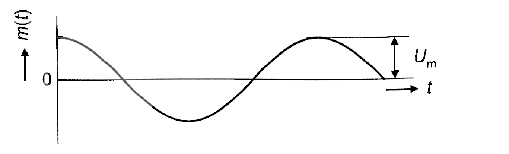
\includegraphics[width=0.8\linewidth]{modulace05_AM.png}}              \\
          \subfloat[harmonická (kosinusová) nosná vlna \(u_c(t)\)]{\label{fig_RA:modulace06}
            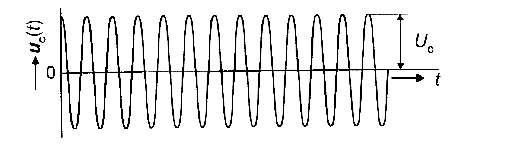
\includegraphics[width=0.8\linewidth]{modulace06_AM.png}}              \\
          \subfloat[odpovídající modulovaný \texttt{AM} signál  
                    \(u_{AM}(t)\)]{\label{fig_RA:modulace07}
            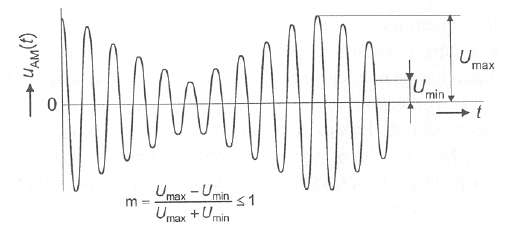
\includegraphics[width=0.8\linewidth]{modulace07_AM.png}}              \\
          \subfloat[kmitočtové spektrum \(F_{AM}(f)\) signálu AM při obecném, neharmonickém  
                    modulačním signálu]{\label{fig_RA:modulace08}
            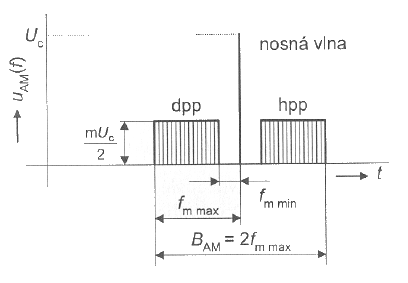
\includegraphics[width=0.7\linewidth]{modulace08_AM.png}}              \\
          \subfloat[fázorová reprezentace signálu \texttt{AM}.]{\label{fig_RA:modulace09} 
            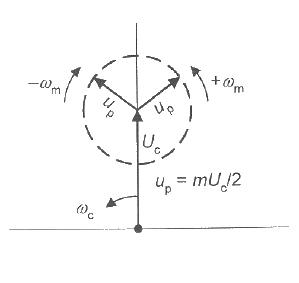
\includegraphics[width=0.7\linewidth]{modulace09_AM.png}}  
        \end{tabular}
        \caption{Podstata amplitudové modulace \texttt{AM}}
      \end{figure}
      
      Amplitudová modulace \texttt{AM} je definována jako modulace, při níž se amplituda nosné vlny 
      mění okolo své střední hodnoty \(U_c\) lineárně s modulačním signálem \(m(t)\). Časový průběh 
      příslušného modulovaného napětí \(u_m(t)\), znázorněného na obr. \ref{fig_RA:modulace07} je 
      tedy dán relací
    
%---------------------------------------------------------------------------------------------------
\printbibliography[heading=subbibliography]
\addcontentsline{toc}{section}{Seznam literatury}